\documentclass[12pt]{article}

\usepackage[spanish]{babel}
\usepackage{hyperref}
\usepackage{graphicx}
\usepackage{listings}
\usepackage{color}
\usepackage{multicol}
\usepackage{amssymb}
\usepackage{enumitem}
\usepackage{here}
\usepackage{dsfont}
\usepackage{amsmath}
\spanishdecimal{.}

\title{Matemáticas para las Ciencias Aplicadas I}
\title{
	Segunda Lista de Problemas \\
	\textbf{Segunda Parte} \\
	\vspace{1ex}
	\large Matemáticas para las Ciencias Aplicadas I \\
	Facultad de Ciencias, UNAM}

\date{\today}

\author{Flores Morán Julieta Melina \\ Zarco Romero José Antonio}

\begin{document}

\maketitle

%% 5, 10, 20, 36 y 40

%% 1
\section{Ejercicio 5} name \\

Utilice una aproximación cuadrática local apropiada para aproximar $\tan 61^{\circ}$ y compare el resultado con el producido directamente por su utilidad de cálculo. \\

A fin de encontrar una fórmula para la aproximación cuadrática local de una función $f$ acerca de $x=x_0$. Esta aproximación tiene la forma:
\[p_2(x)=f(x_0)+f'(x_0)(x-x_0)+\frac{f''(x_0)}{2!}(x-x_0)^2\]
Dado que $61^{\circ} = \frac{\pi}{3} + \frac{\pi}{180} rad$. Entonces, sea $f(x_0)=\tan x_0$ y $x_0=\frac{\pi}{3}$; de este modo:
\begin{center}
\begin{tabular}{r l}
$f(x_0)=\tan x_0$ & $f(\frac{\pi}{3})=\tan \frac{\pi}{3}=\sqrt 3 rad$ \\
$f'(x_0)=(\sec x_0)^2$ & $f'(\frac{\pi}{3})=(\sec \frac{\pi}{3})^2=4 rad$ \\
$f''(x_0)=2 (\sec x_0)^2 \tan x_0$ & $f''(\frac{\pi}{3})=2 (\sec \frac{\pi}{3})^2 \tan \frac{\pi}{3}=8\sqrt 3 rad$ \\
\end{tabular}
\end{center}
Sustituyendo los valores, tenemos que:
\[
p_2(x)=\sqrt 3 + 4(x-\frac{\pi}{3}) + \frac{8 \sqrt 3}{2 \cdot 1}(x-\frac{\pi}{3})^2
=\sqrt 3 + 4(x-\frac{\pi}{3}) + 4 \sqrt 3(x-\frac{\pi}{3})^2
\]
Ya que $x=61^{\circ}=\frac{\pi}{3} + \frac{\pi}{180}rad$
\[
p_2(\frac{\pi}{3} + \frac{\pi}{180}rad)
=\sqrt 3 + 4[(\frac{\pi}{3} + \frac{\pi}{180}rad)-\frac{\pi}{3}] + 4 \sqrt 3[(\frac{\pi}{3} + \frac{\pi}{180}rad)-\frac{\pi}{3}]^2
\]
\[
=\sqrt 3 + 4(\frac{\pi}{180}rad) + 4 \sqrt 3(\frac{\pi}{180}rad)^2
= \sqrt 3 + \frac{\pi}{45}rad + 4 \sqrt 3(\frac{\pi}{180}rad)^2
\]
\[\therefore p_2(61^{\circ}) \approx 1.803974\]
El valor de la aproximación cuadrática local fue de $1.803974$, mientras que el producido directamente por la calculadora fue de $1.804047$.

%% 2
\section{Ejercicio 10} name \\

Encuentre los polinomios de Maclaurin de orden $n = 0, 1, 2, 3, 4$, y luego encuentre los polinomios de Maclaurin enésimos para la función en notación sigma.
\[\sin \pi x\]

Sea $f(x)=\sin \pi x$; de este modo:
\begin{center}
  \begin{tabular}{r l}
    $f(x)=\sin (\pi x)$ & $f(0)=0$ \\
    $f'(x)=\pi \cos (\pi x)$ & $f'(0)=\pi$ \\
    $f''(x)= - \pi ^2 \sin (\pi x)$ & $f''(0)=0$ \\
    $f'''(x)= - \pi ^3 \cos (\pi x)$ & $f'''(0)=-\pi ^3$ \\
    $f^{(4)}(x)= \pi ^4 \sin (\pi x)$ & $f^{(4)}(0)=0$ \\
  \end{tabular}
\end{center}
Dado que el patrón $0, \pi ^k, 0, -\pi ^k$ se repetirá a medida que evaluemos derivadas sucesivas en 0; ya que $f^{(k)}(x)=0$ cuando $k$ es par y, cuando $k$ es impar el resultado de $f^{(k)}(x)$ alterna entre $\pi ^k$ y $-\pi ^k$.
Por lo tanto, los polinomios de Maclaurin de orden $n = 0, 1, 2, 3, 4$ para $\sin \pi x$ son:
\begin{center}
  \begin{tabular}{l}
    $p_0(x)=0$ \\
    $p_1(x)=0+\pi x=\pi x$ \\
    $p_2(x)=0+\pi x+0=\pi x$ \\
    $p_3(x)=0+\pi x+0+\frac{-\pi ^3}{3!}x^3=\pi - \frac{\pi ^3}{3!}x^3=\pi - \frac{\pi ^3}{6}x^3$ \\
    $p_4(x)=0+\pi x+0+\frac{-\pi ^3}{3!}x^3+0=\pi - \frac{\pi ^3}{3!}x^3+0=\pi - \frac{\pi ^3}{6}x^3$ \\
  \end{tabular}
\end{center}

%% 3
\section{Ejercicio 20} name \\

Encuentre los polinomios de Taylor de orden $n = 0, 1, 2, 3, 4$ alrededor de $x = x_0$ y luego encuentre el enésimo polinomio de Taylor para la función en notación sigma.
\[\frac{1}{x+2}\text{; }x_0=3\]

Sea $f(x_0)=\frac{1}{x_0+2}$ y $x_0=3$; de este modo:
\begin{center}
  \begin{tabular}{r l}
    $f(x_0)=\frac{1}{x_0+2}$ & $f(3)=\frac{1}{3+2}=\frac{1}{5}$\\
    $f'(x_0)=-\frac{1}{(x_0+2)^2}$ & $f'(3)=-\frac{1}{(3+2)^2}=-\frac{1}{5^2}=-\frac{1}{25}$\\
    $f''(x_0)=\frac{2}{(x_0+2)^3}$ & $f''(3)=\frac{2}{(3+2)^3}=\frac{2}{5^3}=\frac{2}{125}$\\
    $f'''(x_0)=-\frac{6}{(x_0+2)^4}$ & $f'''(3)=-\frac{6}{(3+2)^4}=-\frac{6}{5^4}=-\frac{6}{625}$ \\
    $f^{(4)}(x_0)=\frac{24}{(x_0+2)^5}$ & $f^{(4)}(3)=\frac{24}{(3+2)^5}=\frac{24}{5^5}=\frac{24}{3125}$ \\
    $\vdots$ & $\vdots$ \\
    $f^{(k)}(x_0)=\sum_{k=0}^{n} (-1)^k \frac{k!}{(x+2)^{k+1}}$ & $f^{(k)}(3)=\sum_{k=0}^{n} (-1)^k \frac{k!}{5^{k+1}}$ \\
  \end{tabular}
\end{center}
Por lo tanto, los polinomios de Taylor de orden $n = 0, 1, 2, 3, 4$ para $f(x)=\frac{1}{x+2}$ alrededor de $x_0 = 3$ son:
\begin{center}
  \begin{tabular}{l}
    $p_0(x)=\frac{1}{5}$ \\
    $p_1(x)=\frac{1}{5}+(-\frac{1}{25})x=\frac{1}{5}-\frac{1}{25}x$ \\
    $p_2(x)=\frac{1}{5}+(-\frac{1}{25})x+\frac{\frac{2}{125}}{2!}(x-3)^2=\frac{1}{5}-\frac{1}{25}x+\frac{1}{125}(x-3)^2$ \\
    $p_3(x)=\frac{1}{5}+(-\frac{1}{25})x+\frac{\frac{2}{125}}{2!}(x-3)^2+\frac{-\frac{6}{625}}{3!}(x-3)^3$ \\
    $=\frac{1}{5}-\frac{1}{25}x+\frac{1}{125}(x-3)^2-\frac{1}{625}(x-3)^3$ \\
    $p_4(x)=\frac{1}{5}+(-\frac{1}{25})x+\frac{\frac{2}{125}}{2!}(x-3)^2+\frac{-\frac{6}{625}}{3!}(x-3)^3+\frac{\frac{24}{3125}}{4!}(x-3)^4$ \\
    $=\frac{1}{5}-\frac{1}{25}x+\frac{1}{125}(x-3)^2-\frac{1}{625}(x-3)^3+\frac{1}{3125}(x-3)^4$ \\
  \end{tabular}
\end{center}
Por tanto, sustituyendo $f^{(k)}(x_0)=\sum_{k=0}^{n} (-1)^k \frac{k!}{5^{k+1}}$ en la fórmula
\[ \sum_{k=0}^{n} \frac{f^{(k)}(x_0)}{k!}(x-x_0)^k \]
Se obtiene el enésimo polinomio de Taylor para la función $\frac{1}{x+2} \text{; } x_0=3$ en notación sigma.
\[
p_n(x)=\sum_{k=0}^{n} \frac{(-1)^k}{5^{k+1}}(x-3)^k
\]

%% 4
\section{Ejercicio 36} name \\

Utilice el método del ejemplo 7 para aproximar la expresión dada a la precisión especificada. Verifique su respuesta con la producida directamente por su utilidad de cálculo.
\[\frac{1}{e}\text{; precisión de tres decimales}\]



%% 5
\section{Ejercicio 40} name \\

\begin{figure}[h!]
\centering
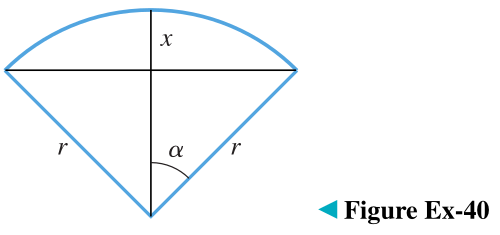
\includegraphics[width=0.5\textwidth]{../img/img_Lista2/2_40.png}
\end{figure}
\begin{enumerate}[label=(\alph*)]
\item La figura adjunta muestra un sector de radio $r$ y ángulo central $2 \alpha$. Suponiendo que el ángulo $\alpha$ es pequeño, utilice la aproximación cuadrática local de $\cos \alpha$ en $\alpha = 0$ para demostrar que $x \approx r \alpha ^2/2$.
\item Suponiendo que la Tierra es una esfera de radio $4000 mi$, use el resultado del inciso $(a)$ para aproximar la cantidad máxima en la que un arco de $100 mi$ a lo largo del ecuador divergirá de su cuerda.
\end{enumerate}

%% 6
\section{Identidad de Euler} name \\

Aplicar las definiciones de las funciones exponencial natural, seno y coseno como series de Taylor para demostrar la identidad de Euler:
\[exp(i\theta) = \cos(\theta) + i \sin(\theta)\]
y deducir, de aquí, que:
\[exp(i\pi) + 1 = 0\]

\end{document}
